%% SECTION HEADER /////////////////////////////////////////////////////////////////////////////////////
\section{Analytical validation of the \ac{pzt} model}
\label{sec:pztVal}

%% SECTION CONTENT ////////////////////////////////////////////////////////////////////////////////////
The current model, i.e. the boundary geometry modelled with the second order elements, is validated by comparing the transducer impedance obtained by numerical simulation and analytical model derived by Giurgiutiu \cite{giurgiutiu2009micromechatronics}.
The impedance Z is a ratio between voltage \((\Phi)\) and current \((I)\) defined as follows:
\begin{eqnarray}
	Z = \frac{\Phi}{I} = \frac{\Phi}{i\omega Q},
\end{eqnarray}
where \(i=\sqrt{-1}\), \(\omega\) is the angular frequency.
In the case of numerical simulation, \(\Phi\) is assumed as the 1.5-cycle Hann windowed sine pulse, and \(Q\) is the charge induced on the electrode calculated by Equation \ref{eq:pzt_sem}. 
The excitation signal has significant values in the 0-300 kHz frequency range, as shown in Fig.~\ref{fig:impedance}(\textbf{a}).
The analytical model is defined as:
\begin{eqnarray}
	Z = \frac{1}{i\omega C_0}\left[\left(1-k_p^2\right)+k_p^2\frac{u_r}{u_I}\right],
\end{eqnarray}
where \(C_0\) is the free capacitance of the sensor, \(k_p\) is the planar coupling coefficient, \(u_r\) is the displacement response, and \(u_I\) is the induced displacement.
Additional, for the comparison, the response of the \ac{sem} with boundary approximation by linear elements was included. 
\begin{figure}[H]
	\begin{center}
		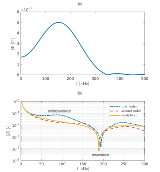
\includegraphics{Chapter_6/impedance}
	\end{center}
	\caption{Validation of the \ac{pzt} model (\textbf{a}) the frequency spectrum of the excitation signal, (\textbf{b}) impedance response of the transducer.}
	\label{fig:impedance}
\end{figure}

It can be notice in Fig.~\ref{fig:impedance}(\textbf{b}) the impedance of the current model is in very good agreement with the analytical solution.
The resonant peak occurred near 190 kHz in both cases, while the resonance of the first-order elements model is shifted 12 kHz toward the higher frequency.
In addition, an antiresonance peak occurred around 90 kHz, not observed in the previous two models.
